

\section{Введение}

% Streams
\subsection{Интерфейс потоков объектов}
\begin{frame}
\frametitle{\insertsection} 
\framesubtitle{\insertsubsection}
% Фича Java 8
% Ленивость
% Функциональный стиль
\begin{itemize}
	\item Java 8 - появление анонимных функций и \textit{java.util.stream}
	\item \textit{java.util.stream} - набор классов и интерфейсов для упрощения обработки последовательностей элементов с помощью функций высших порядков
	\inputminted{java}{code/StreamsExample.java}
	\item Ключевая особенность - ленивость
	\item Аналоги в других языках - LINQ в C\#, коллекции Scala
\end{itemize}
\end{frame}
\subsection{Интерфейс потоков объектов. Реализация}
\begin{frame}
\frametitle{\insertsection} 
\framesubtitle{\insertsubsection}
\begin{itemize}
	\item \textbf{Источник объектов}. Например, массив, коллекция, функция генератор, поток ввода и другие.
	\inputminted{java}{code/Producer.java}
	\item \textbf{Промежуточные операции}. Преобразуют объекты внутри потока.
	\begin{itemize}
		\item Без состояния
		\inputminted{java}{code/Stateless.java}
		\item С состоянием
		\inputminted{java}{code/Stateful.java}
	\end{itemize}
	\item \textbf{Завершающая операция}. Завершает цепочку, преобразуя поток объектов в результат.
	\inputminted{java}{code/Termination.java}
\end{itemize}
\end{frame}

\begin{frame}
\frametitle{\insertsection} 
\framesubtitle{\insertsubsection}
\begin{itemize}
	\item Для повышения производительности потоки примитивных типов имеют отдельную реализацию: $IntStream, LongStream, DoubleStream$.
	\item Существуют расширения $java.util.stream$ - StreamEx, jOOL. Эти библиотеки совместимы со стандартной реализацией, расширяя стандартные интерфейсы.
\end{itemize}
\end{frame}


% Stream debugging
\section{}
\subsection{Отладка потоков объектов}
\begin{frame}
\frametitle{\insertsection} 
\framesubtitle{\insertsubsection}
\begin{itemize}
	\item Точки останова (с условием)
	\item Последовательное исполнение
	\item При помощи метода peek
	\item Конвертация в код с обычными управляющими структурами
	\item Частичное исполнение и сохранение во временную коллекцию
\end{itemize}
\end{frame}

\subsection{Отладка потоков объектов. Недостатки}
\begin{frame}
\frametitle{\insertsection} 
\framesubtitle{\insertsubsection}
Недостатки отладки Stream API в сравнении с обычными управляющими структурами
\begin{itemize}
	\item Нетривиальная последовательность исполнения
	\item Отсутствие знаний о промежуточных результатах вычислений 
	\item Отсутствие информации о трансформации объектов
	\item Сложные стеки вызовов
\end{itemize}

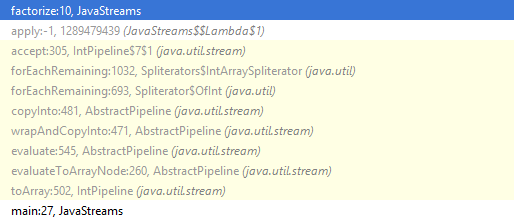
\includegraphics[scale=0.6]{img/stack-trace.png}
\end{frame}

\subsection{Пример использования интерфейса потоков в проекте с открытым кодом}
\begin{frame}
\frametitle{\insertsection} 
\framesubtitle{\insertsubsection}
\inputminted{java}{code/Hard.java}
\end{frame}

\subsection{Существующие решения}
\begin{frame}
\frametitle{\insertsection} 
\framesubtitle{\insertsubsection}
Существует расширение для отладчика Visual Studio для C\# - OzCode. Одна из его функций - отладчик для LINQ.
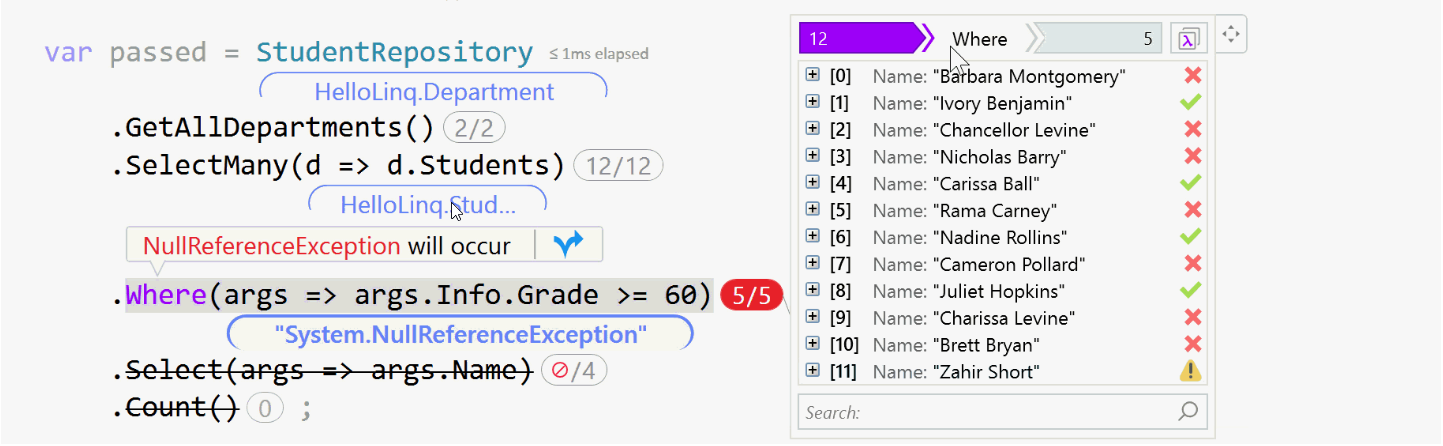
\includegraphics[scale=0.35]{img/ozcode.png}
\end{frame}

\subsection{Особенности OzCode}
\begin{frame}
\frametitle{\insertsection} 
\framesubtitle{\insertsubsection}
\begin{itemize}
	\item Работает с LINQ (язык интегрированных запросов). Его реализация отличается от Stream API в Java
	\item Позволяет увидеть трансформации объектов и промежуточные результаты
	\item Закрытый исходный код
	\item Платный
	\item Только для отладчика Visual Studio
\end{itemize}
\end{frame}

\section{Цель и задачи}
\documentclass[../diploma.tex]{subfiles}
 
\begin{document}

% Теперь мы знаем, как бы мы хотели видеть систему в идеале, осознаем немножко сложность и масштаб области.
% Можно сформулировать задачи, которые я планирую решить в рамках данной работы. 
Сформулируем цели, которые мы ставим в этой работе:

\begin{enumerate}
    \item Реализовать WaveNet максимально придерживаясь описания из статьи.
    \begin{itemize}
        \item Реализовать генерацию голоса без условия.
        \item Реализовать генерацию голоса по тексту.
        \item Реализовать генерацию голоса по тексту с условием.
    \end{itemize}    
\end{enumerate}

Важно отметить, что ключевым аспектом этой подзадачи является педантичная точность в реализации архитектуры сети.
В оригинальной статье архитектура описана довольно высокоуровнево и в общих словах, что подразумевает от читателя уверенных знаний в области и навыков проектирования сетей.

Нам также требуется реализовать дополнительные модификация для локальных и глобальных условий, поскольку они необходимы для генерации с особенностями.

% На самом деле проведя 10 минут в гугле, можно найти большой репозиторий с реализацией WaveNet, вокруг которое даже успело образоваться небольшое комьюнити. У нас ещё такая специфичаная задача, что надо воссоздать архитектуру максимально точно так, как подразумевали создатели, при том, что описали её достаточно высокоуровнево.

% Дело в том, что даже эта реализация далеко не серебянная пуля, так как наша работа очень сильно завиит от того, реализованы ли в сети дополнительные слои, отвечающие за локальный и глобальные условия
% Глобальных условий ещё не было на момент начала работы, а локальные в общем репозитории не появились до сих пор. Поэтому мне их надо реализовать максимально корректно.

\begin{enumerate}[resume]
    \item Разработать признаки для генерации голоса
\end{enumerate}

Требуется спроектировать, реализовать и провести апробацию набора признаков, передаваемых в сеть по каналам локальных и глобальных условий. Авторы WaveNet бегло упоминают используемые признаками, оставляя эту задачу пользователям. 

\begin{enumerate}[resume]
    \item Получить результаты генерации
\end{enumerate}

Наша постановка целей сформулирована так, что мы не можем описать качество работы модели в виде численных измерений.
Поэтому постараемся добиться высокких качеств натуральности голоса в результате экспериментов и получить примеры сгенерированной речи.

% Ну и в конце нужно как-то оценить качественно нащей модели и получить какие-то практические результаты. Как мы увидим после, даже на самом высоком уровне модель содержит много метапараметров.
% Если вдобавок к этому всмопнить, что для хорошей постановки эксперимента нужно подготовить правльний корпус данных да ещё и потратить много машинного времени, в силу высокой требовательнсоти по вычислительным ресурам, то это высрастает в отдельную задачу. 
% Путь не такую сложную интеллектуально или механически как предыдущие две, но требующую много времени и аккуртаности.

\end{document}


\section{Решение}
\subsection{Поиск вызова}
\begin{frame}[noframenumbering]
\frametitle{\insertsection} 
\framesubtitle{\insertsubsection}
Чтобы распознать вызов будем использовать AST файла.
С учетом следующих особенностей:
\begin{itemize}
	\item Определение типа вызова: 
	\begin{itemize}
		\item Источник - первый вызов (объект), возвращающий наследника Stream<T>.
		\item Промежуточный - вызов на наследнике Stream<T>, возвращающий Stream<T>.
		\item Завершающий - вызов на наследнике Stream<T>, возвращающий что-то отличное от Stream<T>.
	\end{itemize}
	\item Цепочка может не иметь завершающей операции. Такие цепочки нам не интересны (в них нет вычислений)
	\item Может быть несколько подходящих вызовов. Необходимо найти их все.
	\item Цепочка может быть на других уровнях стека вызовов.
	\item Цепочка может быть в объемлющем коде.
\end{itemize}
\end{frame}

\subsection{Построение состояний и переходов}
\begin{frame}
\frametitle{\insertsection} 
\framesubtitle{\insertsubsection}
Для отладочных целей интерфейс Stream определяет метод peek.
С помощью него можем запомнить объекты перед и после вызова не изменив логику.
\begin{align*}
	&.peek(x \rightarrow store(x, time)) \\
	&.call(...)\\
	&.peek(z \rightarrow \{time.increment()\})\\
	&.peek(y \rightarrow store(y, time))
\end{align*}

В результате получим два множества $Before = \{(t_i, x_i)\}, After = \{(t_i, y_i)\}$. Они образуют состояния между вызовами.

Чтобы найти переходы достаточно построить \textbf{отображения}
\begin{align*}
	(t_i, x_i) \rightarrow List[(t_j, y_j)], \ \forall (t_i, x_i) \in Before \\
	(t_i, y_i) \rightarrow List[(t_j, x_j)], \ \forall (t_j, y_j) \in After
\end{align*}

\end{frame}

\subsection{Пример}
\begin{frame}
\frametitle{\insertsection} 
\framesubtitle{\insertsubsection}
Рассмотрим в качестве примера вызов:
\inputminted{java}{code/FlatMapFactorizeExample.java}
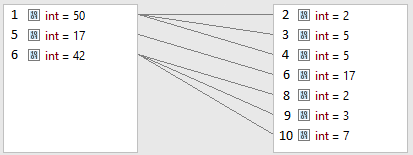
\includegraphics[scale=0.8]{img/flatMapExample.png}

Решая такие же задачи и для остальных методов, получим для них отображение. Такой подход работает почти для всех методов. Исключение - операции с состоянием. Для них можно придумать отдельное решение.
\end{frame}

\subsection{Вычисление}
\begin{frame}
\frametitle{\insertsection} 
\framesubtitle{\insertsubsection}
Выполнение кода трассировки.
\begin{enumerate}
	\item Построить выражение с дополнительными вызовами peek и обработкой собранной информации
	\item Скомпилировать новый класс, в котором будет код, вычисляющий выражение.
	\item Загрузить его в виртуальную машину и выполнить.
	\item Получить результат вычислений и интерпретировать его.
\end{enumerate}
\end{frame}

\subsection{Вычисление. Пример}
\begin{frame}
	\frametitle{\insertsection} 
	\framesubtitle{\insertsubsection}
	\inputminted{java}{code/EvalExample.java}
	Для данной цепочки нужно запустить следующий код.
	\inputminted{java}{code/EvalExampleGenerated.java}
\end{frame}


\section{Результаты}
\begin{frame}
\frametitle{\insertsection} 
\framesubtitle{\insertsubsection}
\begin{itemize}
	\item Разработан плагин, упрощающий отладку операций над потоками объектов.
	\item Плагин размещен в открытом доступе
	\item Поддержаны все операции стандартной реализации Stream API.
	\item Список поддерживаемых методов можно быстро расширить.
\end{itemize}
\end{frame}
 
\begin{frame}
\frametitle{\insertsection} 
\framesubtitle{\insertsubsection}
\href{https://plugins.jetbrains.com/plugin/9696-java-stream-debugger}{https://plugins.jetbrains.com/plugin/9696-java-stream-debugger}

\animategraphics[autoplay,loop,width=\textwidth]{8}{img/demo/demos-}{0}{188}
\end{frame}


\appendix
\section{Архитектура отладчика}
\begin{frame}[noframenumbering]
\frametitle{\insertsection} 
\framesubtitle{\insertsubsection}
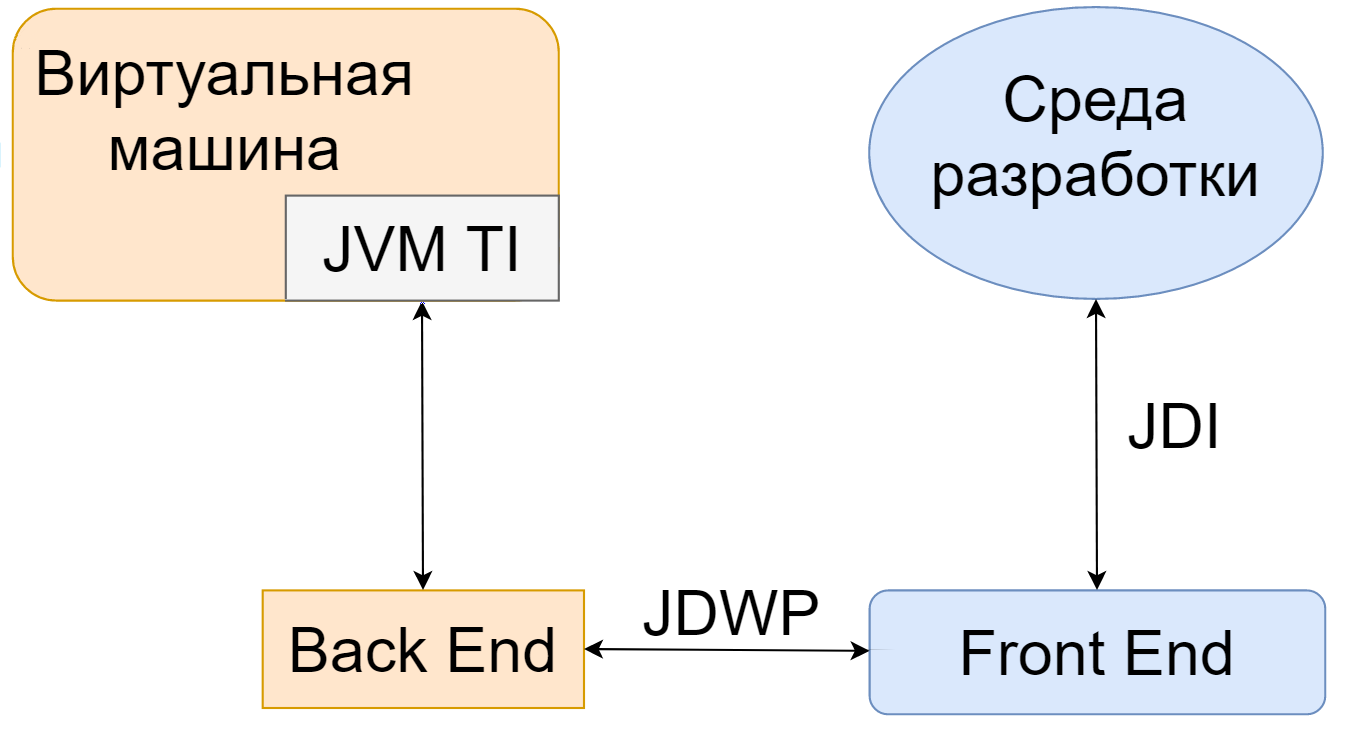
\includegraphics[scale=0.315]{img/jdpa.png}
\end{frame}
\section{Выражение для вычисления}
\begin{frame}[noframenumbering]
\frametitle{\insertsection} 
\framesubtitle{\insertsubsection}
Чтобы вычислить выражение для отслеживания исполнения цепочки потоков объектов нужно определить класс, а так же учесть следующие особенности
\begin{itemize}
	\item Поля и методы этого класса.
	
	\item Расположение класса: пакет, объемлющий класс.
	
	\item Доступ к полям и методам объемлющего класса.

	\item Доступ к приватным членам класса из лямбд и анонимных классов.

	\item Минимизация дальнейших обращений к виртуальной машине.
\end{itemize}

\inputminted{java}{code/EvalClass.java}
\end{frame}

\section{Гарантии библиотеки}
\begin{frame}[noframenumbering]
\frametitle{\insertsection} 
\framesubtitle{\insertsubsection}
Поток объектов всегда ленивый. Это значит, что объекты не из источника будут браться только когда выполняется терминальная операция и ей нужен объект.
\begin{itemize}
	\item Это исключает ситуации, когда из каких-то промежуточных операций требовались объекты, но затем не использовались
	\item Но это не исключает, что некоторым промежуточным операциям потребуется прочитать более одного объекта, чтобы вернуть один. (см sorted, distinct, и др)
	\item Следствие: нет вызова терминальной операции - нет вычислений
\end{itemize}

\end{frame}
\section{Требования к коду пользователя}
\begin{frame}[noframenumbering]
\frametitle{\insertsection} 
\framesubtitle{\insertsubsection}
\begin{itemize}
	\item "Streams are lazy; computation on the source data is only performed when the terminal operation is initiated, and source elements are consumed only as needed."
	\item Это значит, что объекты не могут браться из источника только по необходимости. % ситуация, когда из каких то промежуточных операций забрались объекты, но затем не использовались исключены
	\item Но это не исключает, что некоторым промежуточным операциям потребуется прочитать всё объекты. (см sorted, distinct, и др)
\end{itemize}

\end{frame}
\section{Распознавание вызова}
\begin{frame}[noframenumbering]
\frametitle{\insertsection} 
\framesubtitle{\insertsubsection}
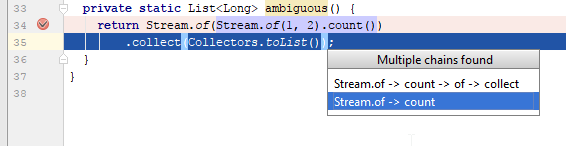
\includegraphics[scale=0.7]{img/ambiguous.png}
\end{frame}


\section{Пример}
\begin{frame}[noframenumbering]
\frametitle{\insertsection} 
\framesubtitle{\insertsubsection}
Рассмотрим пример. Поставим задачу восстановить промежуточные состояния и переходы.
\inputminted{java}{code/StreamWithoutPeeks.java}
\end{frame}

\begin{frame}[noframenumbering]
\frametitle{\insertsection} 
\framesubtitle{\insertsubsection}
Интерфейс Stream определяет для отладочных целей метод peek. Добавим его между всеми вызовами методов Stream<T>.
\inputminted{java}{code/StreamWithPeeks.java}
\end{frame}

\begin{frame}[noframenumbering]
\frametitle{\insertsection} 
\framesubtitle{\insertsubsection}
\fboxsep=0pt
\noindent
	\begin{minipage}[t]{0.48\linewidth}
		Информация, которую можно извлечь:
		\begin{itemize}
			\item Последовательность прохождения объектов через цепочку вызовов
			\item Результат фильтрации
			\item sorted имеет состояние и требует выполнить весь поток до своего вызова
			\item Преобразования объектов
		\end{itemize}
	\end{minipage}
	\hfill%
		\begin{minipage}[t]{0.48\linewidth}
			Результат вызова:
			\inputminted{text}{code/peekResults.txt}
		\end{minipage}
\end{frame}
